\begin{figure}[H]
  \centering
  \begin{subfigure}[t]{.32\linewidth}
    \centering
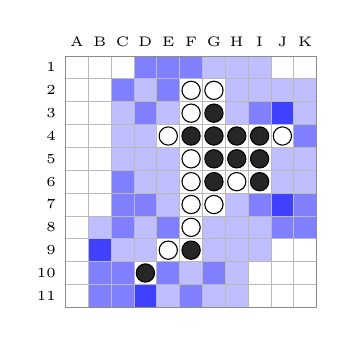
\begin{tikzpicture}[x=0.29cm, y=0.29cm]
\fill[blue!25] (4,-2) rectangle (5,-3);
\fill[blue!75] (3,-10) rectangle (4,-11);
\fill[blue!25] (8,-7) rectangle (9,-8);
\fill[blue!75] (9,-6) rectangle (10,-7);
\fill[blue!50] (2,-7) rectangle (3,-8);
\fill[blue!50] (4,-9) rectangle (5,-10);
\fill[blue!25] (6,-7) rectangle (7,-8);
\fill[blue!75] (1,-8) rectangle (2,-9);
\fill[blue!25] (7,-9) rectangle (8,-10);
\fill[blue!75] (9,-2) rectangle (10,-3);
\fill[blue!25] (1,-7) rectangle (2,-8);
\fill[blue!50] (2,-5) rectangle (3,-6);
\fill[blue!25] (7,-6) rectangle (8,-7);
\fill[blue!25] (9,-5) rectangle (10,-6);
\fill[blue!25] (8,-1) rectangle (9,-2);
\fill[blue!50] (3,-6) rectangle (4,-7);
\fill[blue!50] (3,0) rectangle (4,-1);
\fill[blue!50] (2,-9) rectangle (3,-10);
\fill[blue!50] (1,-9) rectangle (2,-10);
\fill[blue!25] (2,-3) rectangle (3,-4);
\fill[blue!50] (4,-1) rectangle (5,-2);
\fill[blue!50] (8,-6) rectangle (9,-7);
\fill[blue!50] (5,-10) rectangle (6,-11);
\fill[blue!25] (7,0) rectangle (8,-1);
\fill[blue!50] (10,-6) rectangle (11,-7);
\fill[blue!25] (7,-2) rectangle (8,-3);
\fill[blue!50] (8,-2) rectangle (9,-3);
\fill[blue!50] (6,-9) rectangle (7,-10);
\fill[blue!25] (8,-8) rectangle (9,-9);
\fill[blue!25] (2,-4) rectangle (3,-5);
\fill[blue!25] (4,-10) rectangle (5,-11);
\fill[blue!25] (10,-1) rectangle (11,-2);
\fill[blue!50] (3,-2) rectangle (4,-3);
\fill[blue!50] (2,-6) rectangle (3,-7);
\fill[blue!25] (4,-6) rectangle (5,-7);
\fill[blue!25] (6,-10) rectangle (7,-11);
\fill[blue!25] (4,-5) rectangle (5,-6);
\fill[blue!25] (2,-2) rectangle (3,-3);
\fill[blue!25] (10,-4) rectangle (11,-5);
\fill[blue!25] (2,-8) rectangle (3,-9);
\fill[blue!50] (10,-7) rectangle (11,-8);
\fill[blue!25] (7,-8) rectangle (8,-9);
\fill[blue!25] (10,-2) rectangle (11,-3);
\fill[blue!25] (3,-7) rectangle (4,-8);
\fill[blue!25] (6,-8) rectangle (7,-9);
\fill[blue!25] (3,-3) rectangle (4,-4);
\fill[blue!25] (3,-1) rectangle (4,-2);
\fill[blue!50] (10,-3) rectangle (11,-4);
\fill[blue!25] (5,-9) rectangle (6,-10);
\fill[blue!25] (7,-1) rectangle (8,-2);
\fill[blue!25] (9,-1) rectangle (10,-2);
\fill[blue!25] (7,-7) rectangle (8,-8);
\fill[blue!50] (2,-10) rectangle (3,-11);
\fill[blue!50] (5,0) rectangle (6,-1);
\fill[blue!25] (3,-5) rectangle (4,-6);
\fill[blue!25] (4,-4) rectangle (5,-5);
\fill[blue!50] (2,-1) rectangle (3,-2);
\fill[blue!50] (1,-10) rectangle (2,-11);
\fill[blue!25] (7,-10) rectangle (8,-11);
\fill[blue!25] (10,-5) rectangle (11,-6);
\fill[blue!25] (6,0) rectangle (7,-1);
\fill[blue!50] (4,-7) rectangle (5,-8);
\fill[blue!25] (3,-4) rectangle (4,-5);
\fill[blue!25] (8,0) rectangle (9,-1);
\fill[blue!50] (4,0) rectangle (5,-1);
\fill[blue!25] (9,-4) rectangle (10,-5);
\fill[blue!25] (3,-8) rectangle (4,-9);
\fill[blue!50] (9,-7) rectangle (10,-8);
\draw[gray!55, line width=.3pt, step=1] (0,0) grid (11,-11);
\draw[gray!90] (0,0) rectangle (11,-11);
\node[font=\tiny, anchor=south] at (0.5,0) {A};
\node[font=\tiny, anchor=south] at (1.5,0) {B};
\node[font=\tiny, anchor=south] at (2.5,0) {C};
\node[font=\tiny, anchor=south] at (3.5,0) {D};
\node[font=\tiny, anchor=south] at (4.5,0) {E};
\node[font=\tiny, anchor=south] at (5.5,0) {F};
\node[font=\tiny, anchor=south] at (6.5,0) {G};
\node[font=\tiny, anchor=south] at (7.5,0) {H};
\node[font=\tiny, anchor=south] at (8.5,0) {I};
\node[font=\tiny, anchor=south] at (9.5,0) {J};
\node[font=\tiny, anchor=south] at (10.5,0) {K};
\node[font=\tiny, anchor=east] at (0,-0.5) {1};
\node[font=\tiny, anchor=east] at (0,-1.5) {2};
\node[font=\tiny, anchor=east] at (0,-2.5) {3};
\node[font=\tiny, anchor=east] at (0,-3.5) {4};
\node[font=\tiny, anchor=east] at (0,-4.5) {5};
\node[font=\tiny, anchor=east] at (0,-5.5) {6};
\node[font=\tiny, anchor=east] at (0,-6.5) {7};
\node[font=\tiny, anchor=east] at (0,-7.5) {8};
\node[font=\tiny, anchor=east] at (0,-8.5) {9};
\node[font=\tiny, anchor=east] at (0,-9.5) {10};
\node[font=\tiny, anchor=east] at (0,-10.5) {11};
\draw[fill=white, line width=.4pt] (5.5,-1.5) circle (.40);
\draw[fill=white, line width=.4pt] (6.5,-1.5) circle (.40);
\draw[fill=white, line width=.4pt] (5.5,-2.5) circle (.40);
\draw[fill=black!85, line width=.4pt] (6.5,-2.5) circle (.40);
\draw[fill=white, line width=.4pt] (4.5,-3.5) circle (.40);
\draw[fill=black!85, line width=.4pt] (5.5,-3.5) circle (.40);
\draw[fill=black!85, line width=.4pt] (6.5,-3.5) circle (.40);
\draw[fill=black!85, line width=.4pt] (7.5,-3.5) circle (.40);
\draw[fill=black!85, line width=.4pt] (8.5,-3.5) circle (.40);
\draw[fill=white, line width=.4pt] (9.5,-3.5) circle (.40);
\draw[fill=white, line width=.4pt] (5.5,-4.5) circle (.40);
\draw[fill=black!85, line width=.4pt] (6.5,-4.5) circle (.40);
\draw[fill=black!85, line width=.4pt] (7.5,-4.5) circle (.40);
\draw[fill=black!85, line width=.4pt] (8.5,-4.5) circle (.40);
\draw[fill=white, line width=.4pt] (5.5,-5.5) circle (.40);
\draw[fill=black!85, line width=.4pt] (6.5,-5.5) circle (.40);
\draw[fill=white, line width=.4pt] (7.5,-5.5) circle (.40);
\draw[fill=black!85, line width=.4pt] (8.5,-5.5) circle (.40);
\draw[fill=white, line width=.4pt] (5.5,-6.5) circle (.40);
\draw[fill=white, line width=.4pt] (6.5,-6.5) circle (.40);
\draw[fill=white, line width=.4pt] (5.5,-7.5) circle (.40);
\draw[fill=white, line width=.4pt] (4.5,-8.5) circle (.40);
\draw[fill=black!85, line width=.4pt] (5.5,-8.5) circle (.40);
\draw[fill=black!85, line width=.4pt] (3.5,-9.5) circle (.40);
\end{tikzpicture}
    \caption{\footnotesize L4 light, 100: J7}
  \end{subfigure}\hfill
  \begin{subfigure}[t]{.32\linewidth}
    \centering
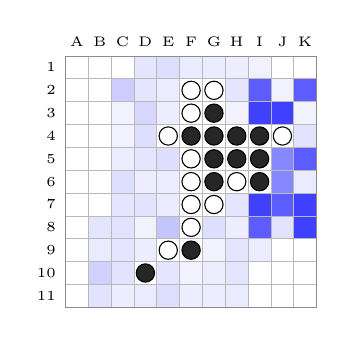
\begin{tikzpicture}[x=0.29cm, y=0.29cm]
\fill[blue!7] (4,-2) rectangle (5,-3);
\fill[blue!8] (3,-10) rectangle (4,-11);
\fill[blue!64] (8,-7) rectangle (9,-8);
\fill[blue!64] (9,-6) rectangle (10,-7);
\fill[blue!11] (2,-7) rectangle (3,-8);
\fill[blue!10] (4,-9) rectangle (5,-10);
\fill[blue!13] (6,-7) rectangle (7,-8);
\fill[blue!8] (1,-8) rectangle (2,-9);
\fill[blue!10] (7,-9) rectangle (8,-10);
\fill[blue!75] (9,-2) rectangle (10,-3);
\fill[blue!10] (1,-7) rectangle (2,-8);
\fill[blue!13] (2,-5) rectangle (3,-6);
\fill[blue!10] (7,-6) rectangle (8,-7);
\fill[blue!47] (9,-5) rectangle (10,-6);
\fill[blue!64] (8,-1) rectangle (9,-2);
\fill[blue!11] (3,-6) rectangle (4,-7);
\fill[blue!10] (3,0) rectangle (4,-1);
\fill[blue!11] (2,-9) rectangle (3,-10);
\fill[blue!18] (1,-9) rectangle (2,-10);
\fill[blue!5] (2,-3) rectangle (3,-4);
\fill[blue!7] (4,-1) rectangle (5,-2);
\fill[blue!75] (8,-6) rectangle (9,-7);
\fill[blue!7] (5,-10) rectangle (6,-11);
\fill[blue!7] (7,0) rectangle (8,-1);
\fill[blue!75] (10,-6) rectangle (11,-7);
\fill[blue!5] (7,-2) rectangle (8,-3);
\fill[blue!75] (8,-2) rectangle (9,-3);
\fill[blue!7] (6,-9) rectangle (7,-10);
\fill[blue!7] (8,-8) rectangle (9,-9);
\fill[blue!7] (2,-4) rectangle (3,-5);
\fill[blue!13] (4,-10) rectangle (5,-11);
\fill[blue!64] (10,-1) rectangle (11,-2);
\fill[blue!16] (3,-2) rectangle (4,-3);
\fill[blue!10] (2,-6) rectangle (3,-7);
\fill[blue!8] (4,-6) rectangle (5,-7);
\fill[blue!7] (6,-10) rectangle (7,-11);
\fill[blue!7] (4,-5) rectangle (5,-6);
\fill[blue!5] (2,-2) rectangle (3,-3);
\fill[blue!64] (10,-4) rectangle (11,-5);
\fill[blue!10] (2,-8) rectangle (3,-9);
\fill[blue!75] (10,-7) rectangle (11,-8);
\fill[blue!10] (7,-8) rectangle (8,-9);
\fill[blue!5] (10,-2) rectangle (11,-3);
\fill[blue!5] (3,-7) rectangle (4,-8);
\fill[blue!5] (6,-8) rectangle (7,-9);
\fill[blue!13] (3,-3) rectangle (4,-4);
\fill[blue!10] (3,-1) rectangle (4,-2);
\fill[blue!11] (10,-3) rectangle (11,-4);
\fill[blue!5] (5,-9) rectangle (6,-10);
\fill[blue!10] (7,-1) rectangle (8,-2);
\fill[blue!5] (9,-1) rectangle (10,-2);
\fill[blue!7] (7,-7) rectangle (8,-8);
\fill[blue!7] (2,-10) rectangle (3,-11);
\fill[blue!8] (5,0) rectangle (6,-1);
\fill[blue!7] (3,-5) rectangle (4,-6);
\fill[blue!13] (4,-4) rectangle (5,-5);
\fill[blue!20] (2,-1) rectangle (3,-2);
\fill[blue!11] (1,-10) rectangle (2,-11);
\fill[blue!8] (7,-10) rectangle (8,-11);
\fill[blue!8] (10,-5) rectangle (11,-6);
\fill[blue!8] (6,0) rectangle (7,-1);
\fill[blue!23] (4,-7) rectangle (5,-8);
\fill[blue!10] (3,-4) rectangle (4,-5);
\fill[blue!5] (8,0) rectangle (9,-1);
\fill[blue!13] (4,0) rectangle (5,-1);
\fill[blue!47] (9,-4) rectangle (10,-5);
\fill[blue!7] (3,-8) rectangle (4,-9);
\fill[blue!11] (9,-7) rectangle (10,-8);
\draw[gray!55, line width=.3pt, step=1] (0,0) grid (11,-11);
\draw[gray!90] (0,0) rectangle (11,-11);
\node[font=\tiny, anchor=south] at (0.5,0) {A};
\node[font=\tiny, anchor=south] at (1.5,0) {B};
\node[font=\tiny, anchor=south] at (2.5,0) {C};
\node[font=\tiny, anchor=south] at (3.5,0) {D};
\node[font=\tiny, anchor=south] at (4.5,0) {E};
\node[font=\tiny, anchor=south] at (5.5,0) {F};
\node[font=\tiny, anchor=south] at (6.5,0) {G};
\node[font=\tiny, anchor=south] at (7.5,0) {H};
\node[font=\tiny, anchor=south] at (8.5,0) {I};
\node[font=\tiny, anchor=south] at (9.5,0) {J};
\node[font=\tiny, anchor=south] at (10.5,0) {K};
\node[font=\tiny, anchor=east] at (0,-0.5) {1};
\node[font=\tiny, anchor=east] at (0,-1.5) {2};
\node[font=\tiny, anchor=east] at (0,-2.5) {3};
\node[font=\tiny, anchor=east] at (0,-3.5) {4};
\node[font=\tiny, anchor=east] at (0,-4.5) {5};
\node[font=\tiny, anchor=east] at (0,-5.5) {6};
\node[font=\tiny, anchor=east] at (0,-6.5) {7};
\node[font=\tiny, anchor=east] at (0,-7.5) {8};
\node[font=\tiny, anchor=east] at (0,-8.5) {9};
\node[font=\tiny, anchor=east] at (0,-9.5) {10};
\node[font=\tiny, anchor=east] at (0,-10.5) {11};
\draw[fill=white, line width=.4pt] (5.5,-1.5) circle (.40);
\draw[fill=white, line width=.4pt] (6.5,-1.5) circle (.40);
\draw[fill=white, line width=.4pt] (5.5,-2.5) circle (.40);
\draw[fill=black!85, line width=.4pt] (6.5,-2.5) circle (.40);
\draw[fill=white, line width=.4pt] (4.5,-3.5) circle (.40);
\draw[fill=black!85, line width=.4pt] (5.5,-3.5) circle (.40);
\draw[fill=black!85, line width=.4pt] (6.5,-3.5) circle (.40);
\draw[fill=black!85, line width=.4pt] (7.5,-3.5) circle (.40);
\draw[fill=black!85, line width=.4pt] (8.5,-3.5) circle (.40);
\draw[fill=white, line width=.4pt] (9.5,-3.5) circle (.40);
\draw[fill=white, line width=.4pt] (5.5,-4.5) circle (.40);
\draw[fill=black!85, line width=.4pt] (6.5,-4.5) circle (.40);
\draw[fill=black!85, line width=.4pt] (7.5,-4.5) circle (.40);
\draw[fill=black!85, line width=.4pt] (8.5,-4.5) circle (.40);
\draw[fill=white, line width=.4pt] (5.5,-5.5) circle (.40);
\draw[fill=black!85, line width=.4pt] (6.5,-5.5) circle (.40);
\draw[fill=white, line width=.4pt] (7.5,-5.5) circle (.40);
\draw[fill=black!85, line width=.4pt] (8.5,-5.5) circle (.40);
\draw[fill=white, line width=.4pt] (5.5,-6.5) circle (.40);
\draw[fill=white, line width=.4pt] (6.5,-6.5) circle (.40);
\draw[fill=white, line width=.4pt] (5.5,-7.5) circle (.40);
\draw[fill=white, line width=.4pt] (4.5,-8.5) circle (.40);
\draw[fill=black!85, line width=.4pt] (5.5,-8.5) circle (.40);
\draw[fill=black!85, line width=.4pt] (3.5,-9.5) circle (.40);
\end{tikzpicture}
    \caption{\footnotesize L4 light, 800: J3}
  \end{subfigure}\hfill
  \begin{subfigure}[t]{.32\linewidth}
    \centering
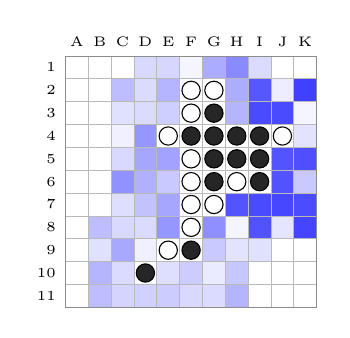
\begin{tikzpicture}[x=0.29cm, y=0.29cm]
\fill[blue!19] (4,-2) rectangle (5,-3);
\fill[blue!18] (3,-10) rectangle (4,-11);
\fill[blue!68] (8,-7) rectangle (9,-8);
\fill[blue!72] (9,-6) rectangle (10,-7);
\fill[blue!15] (2,-7) rectangle (3,-8);
\fill[blue!13] (4,-9) rectangle (5,-10);
\fill[blue!44] (6,-7) rectangle (7,-8);
\fill[blue!12] (1,-8) rectangle (2,-9);
\fill[blue!22] (7,-9) rectangle (8,-10);
\fill[blue!71] (9,-2) rectangle (10,-3);
\fill[blue!26] (1,-7) rectangle (2,-8);
\fill[blue!43] (2,-5) rectangle (3,-6);
\fill[blue!67] (7,-6) rectangle (8,-7);
\fill[blue!68] (9,-5) rectangle (10,-6);
\fill[blue!66] (8,-1) rectangle (9,-2);
\fill[blue!24] (3,-6) rectangle (4,-7);
\fill[blue!15] (3,0) rectangle (4,-1);
\fill[blue!14] (2,-9) rectangle (3,-10);
\fill[blue!29] (1,-9) rectangle (2,-10);
\fill[blue!6] (2,-3) rectangle (3,-4);
\fill[blue!29] (4,-1) rectangle (5,-2);
\fill[blue!71] (8,-6) rectangle (9,-7);
\fill[blue!15] (5,-10) rectangle (6,-11);
\fill[blue!46] (7,0) rectangle (8,-1);
\fill[blue!70] (10,-6) rectangle (11,-7);
\fill[blue!29] (7,-2) rectangle (8,-3);
\fill[blue!71] (8,-2) rectangle (9,-3);
\fill[blue!8] (6,-9) rectangle (7,-10);
\fill[blue!12] (8,-8) rectangle (9,-9);
\fill[blue!15] (2,-4) rectangle (3,-5);
\fill[blue!20] (4,-10) rectangle (5,-11);
\fill[blue!75] (10,-1) rectangle (11,-2);
\fill[blue!14] (3,-2) rectangle (4,-3);
\fill[blue!13] (2,-6) rectangle (3,-7);
\fill[blue!35] (4,-6) rectangle (5,-7);
\fill[blue!14] (6,-10) rectangle (7,-11);
\fill[blue!21] (4,-5) rectangle (5,-6);
\fill[blue!12] (2,-2) rectangle (3,-3);
\fill[blue!69] (10,-4) rectangle (11,-5);
\fill[blue!34] (2,-8) rectangle (3,-9);
\fill[blue!73] (10,-7) rectangle (11,-8);
\fill[blue!11] (7,-8) rectangle (8,-9);
\fill[blue!4] (10,-2) rectangle (11,-3);
\fill[blue!14] (3,-7) rectangle (4,-8);
\fill[blue!21] (6,-8) rectangle (7,-9);
\fill[blue!41] (3,-3) rectangle (4,-4);
\fill[blue!14] (3,-1) rectangle (4,-2);
\fill[blue!11] (10,-3) rectangle (11,-4);
\fill[blue!20] (5,-9) rectangle (6,-10);
\fill[blue!32] (7,-1) rectangle (8,-2);
\fill[blue!7] (9,-1) rectangle (10,-2);
\fill[blue!4] (7,-7) rectangle (8,-8);
\fill[blue!17] (2,-10) rectangle (3,-11);
\fill[blue!4] (5,0) rectangle (6,-1);
\fill[blue!31] (3,-5) rectangle (4,-6);
\fill[blue!36] (4,-4) rectangle (5,-5);
\fill[blue!26] (2,-1) rectangle (3,-2);
\fill[blue!26] (1,-10) rectangle (2,-11);
\fill[blue!29] (7,-10) rectangle (8,-11);
\fill[blue!21] (10,-5) rectangle (11,-6);
\fill[blue!33] (6,0) rectangle (7,-1);
\fill[blue!41] (4,-7) rectangle (5,-8);
\fill[blue!35] (3,-4) rectangle (4,-5);
\fill[blue!14] (8,0) rectangle (9,-1);
\fill[blue!16] (4,0) rectangle (5,-1);
\fill[blue!67] (9,-4) rectangle (10,-5);
\fill[blue!6] (3,-8) rectangle (4,-9);
\fill[blue!10] (9,-7) rectangle (10,-8);
\draw[gray!55, line width=.3pt, step=1] (0,0) grid (11,-11);
\draw[gray!90] (0,0) rectangle (11,-11);
\node[font=\tiny, anchor=south] at (0.5,0) {A};
\node[font=\tiny, anchor=south] at (1.5,0) {B};
\node[font=\tiny, anchor=south] at (2.5,0) {C};
\node[font=\tiny, anchor=south] at (3.5,0) {D};
\node[font=\tiny, anchor=south] at (4.5,0) {E};
\node[font=\tiny, anchor=south] at (5.5,0) {F};
\node[font=\tiny, anchor=south] at (6.5,0) {G};
\node[font=\tiny, anchor=south] at (7.5,0) {H};
\node[font=\tiny, anchor=south] at (8.5,0) {I};
\node[font=\tiny, anchor=south] at (9.5,0) {J};
\node[font=\tiny, anchor=south] at (10.5,0) {K};
\node[font=\tiny, anchor=east] at (0,-0.5) {1};
\node[font=\tiny, anchor=east] at (0,-1.5) {2};
\node[font=\tiny, anchor=east] at (0,-2.5) {3};
\node[font=\tiny, anchor=east] at (0,-3.5) {4};
\node[font=\tiny, anchor=east] at (0,-4.5) {5};
\node[font=\tiny, anchor=east] at (0,-5.5) {6};
\node[font=\tiny, anchor=east] at (0,-6.5) {7};
\node[font=\tiny, anchor=east] at (0,-7.5) {8};
\node[font=\tiny, anchor=east] at (0,-8.5) {9};
\node[font=\tiny, anchor=east] at (0,-9.5) {10};
\node[font=\tiny, anchor=east] at (0,-10.5) {11};
\draw[fill=white, line width=.4pt] (5.5,-1.5) circle (.40);
\draw[fill=white, line width=.4pt] (6.5,-1.5) circle (.40);
\draw[fill=white, line width=.4pt] (5.5,-2.5) circle (.40);
\draw[fill=black!85, line width=.4pt] (6.5,-2.5) circle (.40);
\draw[fill=white, line width=.4pt] (4.5,-3.5) circle (.40);
\draw[fill=black!85, line width=.4pt] (5.5,-3.5) circle (.40);
\draw[fill=black!85, line width=.4pt] (6.5,-3.5) circle (.40);
\draw[fill=black!85, line width=.4pt] (7.5,-3.5) circle (.40);
\draw[fill=black!85, line width=.4pt] (8.5,-3.5) circle (.40);
\draw[fill=white, line width=.4pt] (9.5,-3.5) circle (.40);
\draw[fill=white, line width=.4pt] (5.5,-4.5) circle (.40);
\draw[fill=black!85, line width=.4pt] (6.5,-4.5) circle (.40);
\draw[fill=black!85, line width=.4pt] (7.5,-4.5) circle (.40);
\draw[fill=black!85, line width=.4pt] (8.5,-4.5) circle (.40);
\draw[fill=white, line width=.4pt] (5.5,-5.5) circle (.40);
\draw[fill=black!85, line width=.4pt] (6.5,-5.5) circle (.40);
\draw[fill=white, line width=.4pt] (7.5,-5.5) circle (.40);
\draw[fill=black!85, line width=.4pt] (8.5,-5.5) circle (.40);
\draw[fill=white, line width=.4pt] (5.5,-6.5) circle (.40);
\draw[fill=white, line width=.4pt] (6.5,-6.5) circle (.40);
\draw[fill=white, line width=.4pt] (5.5,-7.5) circle (.40);
\draw[fill=white, line width=.4pt] (4.5,-8.5) circle (.40);
\draw[fill=black!85, line width=.4pt] (5.5,-8.5) circle (.40);
\draw[fill=black!85, line width=.4pt] (3.5,-9.5) circle (.40);
\end{tikzpicture}
    \caption{\footnotesize L4 light, 6.400: K2}
  \end{subfigure}\par\medskip
  \begin{subfigure}[t]{.32\linewidth}
    \centering
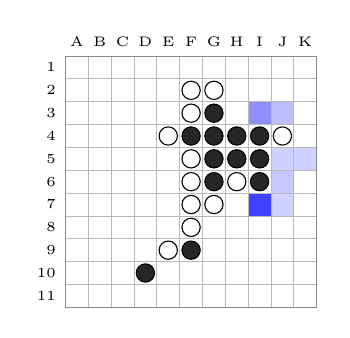
\begin{tikzpicture}[x=0.29cm, y=0.29cm]
\fill[blue!44] (8,-2) rectangle (9,-3);
\fill[blue!26] (9,-2) rectangle (10,-3);
\fill[blue!18] (9,-4) rectangle (10,-5);
\fill[blue!18] (10,-4) rectangle (11,-5);
\fill[blue!22] (9,-5) rectangle (10,-6);
\fill[blue!75] (8,-6) rectangle (9,-7);
\fill[blue!18] (9,-6) rectangle (10,-7);
\draw[gray!55, line width=.3pt, step=1] (0,0) grid (11,-11);
\draw[gray!90] (0,0) rectangle (11,-11);
\node[font=\tiny, anchor=south] at (0.5,0) {A};
\node[font=\tiny, anchor=south] at (1.5,0) {B};
\node[font=\tiny, anchor=south] at (2.5,0) {C};
\node[font=\tiny, anchor=south] at (3.5,0) {D};
\node[font=\tiny, anchor=south] at (4.5,0) {E};
\node[font=\tiny, anchor=south] at (5.5,0) {F};
\node[font=\tiny, anchor=south] at (6.5,0) {G};
\node[font=\tiny, anchor=south] at (7.5,0) {H};
\node[font=\tiny, anchor=south] at (8.5,0) {I};
\node[font=\tiny, anchor=south] at (9.5,0) {J};
\node[font=\tiny, anchor=south] at (10.5,0) {K};
\node[font=\tiny, anchor=east] at (0,-0.5) {1};
\node[font=\tiny, anchor=east] at (0,-1.5) {2};
\node[font=\tiny, anchor=east] at (0,-2.5) {3};
\node[font=\tiny, anchor=east] at (0,-3.5) {4};
\node[font=\tiny, anchor=east] at (0,-4.5) {5};
\node[font=\tiny, anchor=east] at (0,-5.5) {6};
\node[font=\tiny, anchor=east] at (0,-6.5) {7};
\node[font=\tiny, anchor=east] at (0,-7.5) {8};
\node[font=\tiny, anchor=east] at (0,-8.5) {9};
\node[font=\tiny, anchor=east] at (0,-9.5) {10};
\node[font=\tiny, anchor=east] at (0,-10.5) {11};
\draw[fill=white, line width=.4pt] (5.5,-1.5) circle (.40);
\draw[fill=white, line width=.4pt] (6.5,-1.5) circle (.40);
\draw[fill=white, line width=.4pt] (5.5,-2.5) circle (.40);
\draw[fill=black!85, line width=.4pt] (6.5,-2.5) circle (.40);
\draw[fill=white, line width=.4pt] (4.5,-3.5) circle (.40);
\draw[fill=black!85, line width=.4pt] (5.5,-3.5) circle (.40);
\draw[fill=black!85, line width=.4pt] (6.5,-3.5) circle (.40);
\draw[fill=black!85, line width=.4pt] (7.5,-3.5) circle (.40);
\draw[fill=black!85, line width=.4pt] (8.5,-3.5) circle (.40);
\draw[fill=white, line width=.4pt] (9.5,-3.5) circle (.40);
\draw[fill=white, line width=.4pt] (5.5,-4.5) circle (.40);
\draw[fill=black!85, line width=.4pt] (6.5,-4.5) circle (.40);
\draw[fill=black!85, line width=.4pt] (7.5,-4.5) circle (.40);
\draw[fill=black!85, line width=.4pt] (8.5,-4.5) circle (.40);
\draw[fill=white, line width=.4pt] (5.5,-5.5) circle (.40);
\draw[fill=black!85, line width=.4pt] (6.5,-5.5) circle (.40);
\draw[fill=white, line width=.4pt] (7.5,-5.5) circle (.40);
\draw[fill=black!85, line width=.4pt] (8.5,-5.5) circle (.40);
\draw[fill=white, line width=.4pt] (5.5,-6.5) circle (.40);
\draw[fill=white, line width=.4pt] (6.5,-6.5) circle (.40);
\draw[fill=white, line width=.4pt] (5.5,-7.5) circle (.40);
\draw[fill=white, line width=.4pt] (4.5,-8.5) circle (.40);
\draw[fill=black!85, line width=.4pt] (5.5,-8.5) circle (.40);
\draw[fill=black!85, line width=.4pt] (3.5,-9.5) circle (.40);
\end{tikzpicture}
    \caption{\footnotesize L7, 50: I7}
  \end{subfigure}\hfill
  \begin{subfigure}[t]{.32\linewidth}
    \centering
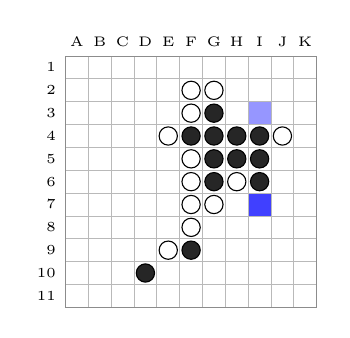
\begin{tikzpicture}[x=0.29cm, y=0.29cm]
\fill[blue!41] (8,-2) rectangle (9,-3);
\fill[blue!75] (8,-6) rectangle (9,-7);
\draw[gray!55, line width=.3pt, step=1] (0,0) grid (11,-11);
\draw[gray!90] (0,0) rectangle (11,-11);
\node[font=\tiny, anchor=south] at (0.5,0) {A};
\node[font=\tiny, anchor=south] at (1.5,0) {B};
\node[font=\tiny, anchor=south] at (2.5,0) {C};
\node[font=\tiny, anchor=south] at (3.5,0) {D};
\node[font=\tiny, anchor=south] at (4.5,0) {E};
\node[font=\tiny, anchor=south] at (5.5,0) {F};
\node[font=\tiny, anchor=south] at (6.5,0) {G};
\node[font=\tiny, anchor=south] at (7.5,0) {H};
\node[font=\tiny, anchor=south] at (8.5,0) {I};
\node[font=\tiny, anchor=south] at (9.5,0) {J};
\node[font=\tiny, anchor=south] at (10.5,0) {K};
\node[font=\tiny, anchor=east] at (0,-0.5) {1};
\node[font=\tiny, anchor=east] at (0,-1.5) {2};
\node[font=\tiny, anchor=east] at (0,-2.5) {3};
\node[font=\tiny, anchor=east] at (0,-3.5) {4};
\node[font=\tiny, anchor=east] at (0,-4.5) {5};
\node[font=\tiny, anchor=east] at (0,-5.5) {6};
\node[font=\tiny, anchor=east] at (0,-6.5) {7};
\node[font=\tiny, anchor=east] at (0,-7.5) {8};
\node[font=\tiny, anchor=east] at (0,-8.5) {9};
\node[font=\tiny, anchor=east] at (0,-9.5) {10};
\node[font=\tiny, anchor=east] at (0,-10.5) {11};
\draw[fill=white, line width=.4pt] (5.5,-1.5) circle (.40);
\draw[fill=white, line width=.4pt] (6.5,-1.5) circle (.40);
\draw[fill=white, line width=.4pt] (5.5,-2.5) circle (.40);
\draw[fill=black!85, line width=.4pt] (6.5,-2.5) circle (.40);
\draw[fill=white, line width=.4pt] (4.5,-3.5) circle (.40);
\draw[fill=black!85, line width=.4pt] (5.5,-3.5) circle (.40);
\draw[fill=black!85, line width=.4pt] (6.5,-3.5) circle (.40);
\draw[fill=black!85, line width=.4pt] (7.5,-3.5) circle (.40);
\draw[fill=black!85, line width=.4pt] (8.5,-3.5) circle (.40);
\draw[fill=white, line width=.4pt] (9.5,-3.5) circle (.40);
\draw[fill=white, line width=.4pt] (5.5,-4.5) circle (.40);
\draw[fill=black!85, line width=.4pt] (6.5,-4.5) circle (.40);
\draw[fill=black!85, line width=.4pt] (7.5,-4.5) circle (.40);
\draw[fill=black!85, line width=.4pt] (8.5,-4.5) circle (.40);
\draw[fill=white, line width=.4pt] (5.5,-5.5) circle (.40);
\draw[fill=black!85, line width=.4pt] (6.5,-5.5) circle (.40);
\draw[fill=white, line width=.4pt] (7.5,-5.5) circle (.40);
\draw[fill=black!85, line width=.4pt] (8.5,-5.5) circle (.40);
\draw[fill=white, line width=.4pt] (5.5,-6.5) circle (.40);
\draw[fill=white, line width=.4pt] (6.5,-6.5) circle (.40);
\draw[fill=white, line width=.4pt] (5.5,-7.5) circle (.40);
\draw[fill=white, line width=.4pt] (4.5,-8.5) circle (.40);
\draw[fill=black!85, line width=.4pt] (5.5,-8.5) circle (.40);
\draw[fill=black!85, line width=.4pt] (3.5,-9.5) circle (.40);
\end{tikzpicture}
    \caption{\footnotesize L7, 800: I7}
  \end{subfigure}\hfill
  \begin{subfigure}[t]{.32\linewidth}
    \centering
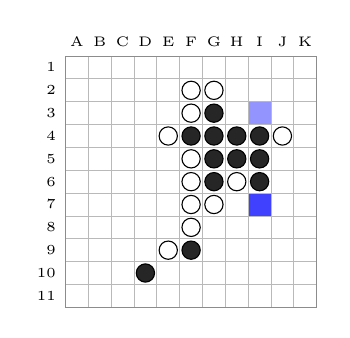
\begin{tikzpicture}[x=0.29cm, y=0.29cm]
\fill[blue!42] (8,-2) rectangle (9,-3);
\fill[blue!75] (8,-6) rectangle (9,-7);
\draw[gray!55, line width=.3pt, step=1] (0,0) grid (11,-11);
\draw[gray!90] (0,0) rectangle (11,-11);
\node[font=\tiny, anchor=south] at (0.5,0) {A};
\node[font=\tiny, anchor=south] at (1.5,0) {B};
\node[font=\tiny, anchor=south] at (2.5,0) {C};
\node[font=\tiny, anchor=south] at (3.5,0) {D};
\node[font=\tiny, anchor=south] at (4.5,0) {E};
\node[font=\tiny, anchor=south] at (5.5,0) {F};
\node[font=\tiny, anchor=south] at (6.5,0) {G};
\node[font=\tiny, anchor=south] at (7.5,0) {H};
\node[font=\tiny, anchor=south] at (8.5,0) {I};
\node[font=\tiny, anchor=south] at (9.5,0) {J};
\node[font=\tiny, anchor=south] at (10.5,0) {K};
\node[font=\tiny, anchor=east] at (0,-0.5) {1};
\node[font=\tiny, anchor=east] at (0,-1.5) {2};
\node[font=\tiny, anchor=east] at (0,-2.5) {3};
\node[font=\tiny, anchor=east] at (0,-3.5) {4};
\node[font=\tiny, anchor=east] at (0,-4.5) {5};
\node[font=\tiny, anchor=east] at (0,-5.5) {6};
\node[font=\tiny, anchor=east] at (0,-6.5) {7};
\node[font=\tiny, anchor=east] at (0,-7.5) {8};
\node[font=\tiny, anchor=east] at (0,-8.5) {9};
\node[font=\tiny, anchor=east] at (0,-9.5) {10};
\node[font=\tiny, anchor=east] at (0,-10.5) {11};
\draw[fill=white, line width=.4pt] (5.5,-1.5) circle (.40);
\draw[fill=white, line width=.4pt] (6.5,-1.5) circle (.40);
\draw[fill=white, line width=.4pt] (5.5,-2.5) circle (.40);
\draw[fill=black!85, line width=.4pt] (6.5,-2.5) circle (.40);
\draw[fill=white, line width=.4pt] (4.5,-3.5) circle (.40);
\draw[fill=black!85, line width=.4pt] (5.5,-3.5) circle (.40);
\draw[fill=black!85, line width=.4pt] (6.5,-3.5) circle (.40);
\draw[fill=black!85, line width=.4pt] (7.5,-3.5) circle (.40);
\draw[fill=black!85, line width=.4pt] (8.5,-3.5) circle (.40);
\draw[fill=white, line width=.4pt] (9.5,-3.5) circle (.40);
\draw[fill=white, line width=.4pt] (5.5,-4.5) circle (.40);
\draw[fill=black!85, line width=.4pt] (6.5,-4.5) circle (.40);
\draw[fill=black!85, line width=.4pt] (7.5,-4.5) circle (.40);
\draw[fill=black!85, line width=.4pt] (8.5,-4.5) circle (.40);
\draw[fill=white, line width=.4pt] (5.5,-5.5) circle (.40);
\draw[fill=black!85, line width=.4pt] (6.5,-5.5) circle (.40);
\draw[fill=white, line width=.4pt] (7.5,-5.5) circle (.40);
\draw[fill=black!85, line width=.4pt] (8.5,-5.5) circle (.40);
\draw[fill=white, line width=.4pt] (5.5,-6.5) circle (.40);
\draw[fill=white, line width=.4pt] (6.5,-6.5) circle (.40);
\draw[fill=white, line width=.4pt] (5.5,-7.5) circle (.40);
\draw[fill=white, line width=.4pt] (4.5,-8.5) circle (.40);
\draw[fill=black!85, line width=.4pt] (5.5,-8.5) circle (.40);
\draw[fill=black!85, line width=.4pt] (3.5,-9.5) circle (.40);
\end{tikzpicture}
    \caption{\footnotesize L7, 3.200: I7}
  \end{subfigure}\par\medskip
  \begin{subfigure}[t]{.32\linewidth}
    \centering
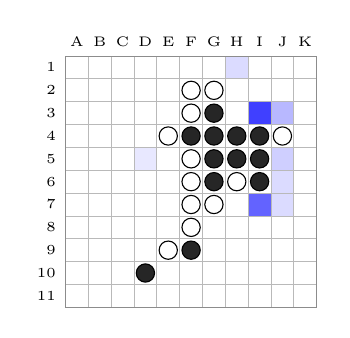
\begin{tikzpicture}[x=0.29cm, y=0.29cm]
\fill[blue!14] (7,0) rectangle (8,-1);
\fill[blue!75] (8,-2) rectangle (9,-3);
\fill[blue!28] (9,-2) rectangle (10,-3);
\fill[blue!9] (3,-4) rectangle (4,-5);
\fill[blue!19] (9,-4) rectangle (10,-5);
\fill[blue!14] (9,-5) rectangle (10,-6);
\fill[blue!61] (8,-6) rectangle (9,-7);
\fill[blue!14] (9,-6) rectangle (10,-7);
\draw[gray!55, line width=.3pt, step=1] (0,0) grid (11,-11);
\draw[gray!90] (0,0) rectangle (11,-11);
\node[font=\tiny, anchor=south] at (0.5,0) {A};
\node[font=\tiny, anchor=south] at (1.5,0) {B};
\node[font=\tiny, anchor=south] at (2.5,0) {C};
\node[font=\tiny, anchor=south] at (3.5,0) {D};
\node[font=\tiny, anchor=south] at (4.5,0) {E};
\node[font=\tiny, anchor=south] at (5.5,0) {F};
\node[font=\tiny, anchor=south] at (6.5,0) {G};
\node[font=\tiny, anchor=south] at (7.5,0) {H};
\node[font=\tiny, anchor=south] at (8.5,0) {I};
\node[font=\tiny, anchor=south] at (9.5,0) {J};
\node[font=\tiny, anchor=south] at (10.5,0) {K};
\node[font=\tiny, anchor=east] at (0,-0.5) {1};
\node[font=\tiny, anchor=east] at (0,-1.5) {2};
\node[font=\tiny, anchor=east] at (0,-2.5) {3};
\node[font=\tiny, anchor=east] at (0,-3.5) {4};
\node[font=\tiny, anchor=east] at (0,-4.5) {5};
\node[font=\tiny, anchor=east] at (0,-5.5) {6};
\node[font=\tiny, anchor=east] at (0,-6.5) {7};
\node[font=\tiny, anchor=east] at (0,-7.5) {8};
\node[font=\tiny, anchor=east] at (0,-8.5) {9};
\node[font=\tiny, anchor=east] at (0,-9.5) {10};
\node[font=\tiny, anchor=east] at (0,-10.5) {11};
\draw[fill=white, line width=.4pt] (5.5,-1.5) circle (.40);
\draw[fill=white, line width=.4pt] (6.5,-1.5) circle (.40);
\draw[fill=white, line width=.4pt] (5.5,-2.5) circle (.40);
\draw[fill=black!85, line width=.4pt] (6.5,-2.5) circle (.40);
\draw[fill=white, line width=.4pt] (4.5,-3.5) circle (.40);
\draw[fill=black!85, line width=.4pt] (5.5,-3.5) circle (.40);
\draw[fill=black!85, line width=.4pt] (6.5,-3.5) circle (.40);
\draw[fill=black!85, line width=.4pt] (7.5,-3.5) circle (.40);
\draw[fill=black!85, line width=.4pt] (8.5,-3.5) circle (.40);
\draw[fill=white, line width=.4pt] (9.5,-3.5) circle (.40);
\draw[fill=white, line width=.4pt] (5.5,-4.5) circle (.40);
\draw[fill=black!85, line width=.4pt] (6.5,-4.5) circle (.40);
\draw[fill=black!85, line width=.4pt] (7.5,-4.5) circle (.40);
\draw[fill=black!85, line width=.4pt] (8.5,-4.5) circle (.40);
\draw[fill=white, line width=.4pt] (5.5,-5.5) circle (.40);
\draw[fill=black!85, line width=.4pt] (6.5,-5.5) circle (.40);
\draw[fill=white, line width=.4pt] (7.5,-5.5) circle (.40);
\draw[fill=black!85, line width=.4pt] (8.5,-5.5) circle (.40);
\draw[fill=white, line width=.4pt] (5.5,-6.5) circle (.40);
\draw[fill=white, line width=.4pt] (6.5,-6.5) circle (.40);
\draw[fill=white, line width=.4pt] (5.5,-7.5) circle (.40);
\draw[fill=white, line width=.4pt] (4.5,-8.5) circle (.40);
\draw[fill=black!85, line width=.4pt] (5.5,-8.5) circle (.40);
\draw[fill=black!85, line width=.4pt] (3.5,-9.5) circle (.40);
\end{tikzpicture}
    \caption{\footnotesize L8, 50: I3}
  \end{subfigure}\hfill
  \begin{subfigure}[t]{.32\linewidth}
    \centering
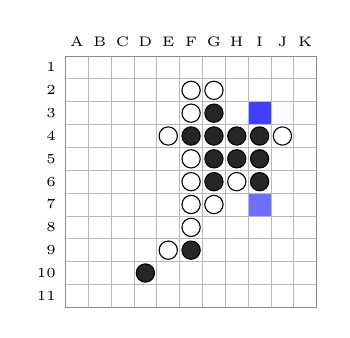
\begin{tikzpicture}[x=0.29cm, y=0.29cm]
\fill[blue!75] (8,-2) rectangle (9,-3);
\fill[blue!2] (9,-2) rectangle (10,-3);
\fill[blue!57] (8,-6) rectangle (9,-7);
\draw[gray!55, line width=.3pt, step=1] (0,0) grid (11,-11);
\draw[gray!90] (0,0) rectangle (11,-11);
\node[font=\tiny, anchor=south] at (0.5,0) {A};
\node[font=\tiny, anchor=south] at (1.5,0) {B};
\node[font=\tiny, anchor=south] at (2.5,0) {C};
\node[font=\tiny, anchor=south] at (3.5,0) {D};
\node[font=\tiny, anchor=south] at (4.5,0) {E};
\node[font=\tiny, anchor=south] at (5.5,0) {F};
\node[font=\tiny, anchor=south] at (6.5,0) {G};
\node[font=\tiny, anchor=south] at (7.5,0) {H};
\node[font=\tiny, anchor=south] at (8.5,0) {I};
\node[font=\tiny, anchor=south] at (9.5,0) {J};
\node[font=\tiny, anchor=south] at (10.5,0) {K};
\node[font=\tiny, anchor=east] at (0,-0.5) {1};
\node[font=\tiny, anchor=east] at (0,-1.5) {2};
\node[font=\tiny, anchor=east] at (0,-2.5) {3};
\node[font=\tiny, anchor=east] at (0,-3.5) {4};
\node[font=\tiny, anchor=east] at (0,-4.5) {5};
\node[font=\tiny, anchor=east] at (0,-5.5) {6};
\node[font=\tiny, anchor=east] at (0,-6.5) {7};
\node[font=\tiny, anchor=east] at (0,-7.5) {8};
\node[font=\tiny, anchor=east] at (0,-8.5) {9};
\node[font=\tiny, anchor=east] at (0,-9.5) {10};
\node[font=\tiny, anchor=east] at (0,-10.5) {11};
\draw[fill=white, line width=.4pt] (5.5,-1.5) circle (.40);
\draw[fill=white, line width=.4pt] (6.5,-1.5) circle (.40);
\draw[fill=white, line width=.4pt] (5.5,-2.5) circle (.40);
\draw[fill=black!85, line width=.4pt] (6.5,-2.5) circle (.40);
\draw[fill=white, line width=.4pt] (4.5,-3.5) circle (.40);
\draw[fill=black!85, line width=.4pt] (5.5,-3.5) circle (.40);
\draw[fill=black!85, line width=.4pt] (6.5,-3.5) circle (.40);
\draw[fill=black!85, line width=.4pt] (7.5,-3.5) circle (.40);
\draw[fill=black!85, line width=.4pt] (8.5,-3.5) circle (.40);
\draw[fill=white, line width=.4pt] (9.5,-3.5) circle (.40);
\draw[fill=white, line width=.4pt] (5.5,-4.5) circle (.40);
\draw[fill=black!85, line width=.4pt] (6.5,-4.5) circle (.40);
\draw[fill=black!85, line width=.4pt] (7.5,-4.5) circle (.40);
\draw[fill=black!85, line width=.4pt] (8.5,-4.5) circle (.40);
\draw[fill=white, line width=.4pt] (5.5,-5.5) circle (.40);
\draw[fill=black!85, line width=.4pt] (6.5,-5.5) circle (.40);
\draw[fill=white, line width=.4pt] (7.5,-5.5) circle (.40);
\draw[fill=black!85, line width=.4pt] (8.5,-5.5) circle (.40);
\draw[fill=white, line width=.4pt] (5.5,-6.5) circle (.40);
\draw[fill=white, line width=.4pt] (6.5,-6.5) circle (.40);
\draw[fill=white, line width=.4pt] (5.5,-7.5) circle (.40);
\draw[fill=white, line width=.4pt] (4.5,-8.5) circle (.40);
\draw[fill=black!85, line width=.4pt] (5.5,-8.5) circle (.40);
\draw[fill=black!85, line width=.4pt] (3.5,-9.5) circle (.40);
\end{tikzpicture}
    \caption{\footnotesize L8, 800: I3}
  \end{subfigure}\hfill
  \begin{subfigure}[t]{.32\linewidth}
    \centering
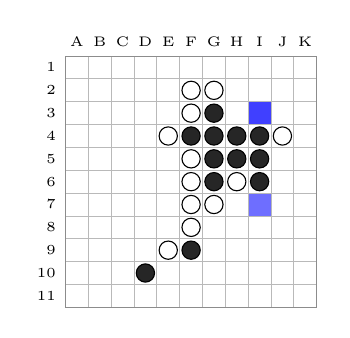
\begin{tikzpicture}[x=0.29cm, y=0.29cm]
\fill[blue!75] (8,-2) rectangle (9,-3);
\fill[blue!57] (8,-6) rectangle (9,-7);
\draw[gray!55, line width=.3pt, step=1] (0,0) grid (11,-11);
\draw[gray!90] (0,0) rectangle (11,-11);
\node[font=\tiny, anchor=south] at (0.5,0) {A};
\node[font=\tiny, anchor=south] at (1.5,0) {B};
\node[font=\tiny, anchor=south] at (2.5,0) {C};
\node[font=\tiny, anchor=south] at (3.5,0) {D};
\node[font=\tiny, anchor=south] at (4.5,0) {E};
\node[font=\tiny, anchor=south] at (5.5,0) {F};
\node[font=\tiny, anchor=south] at (6.5,0) {G};
\node[font=\tiny, anchor=south] at (7.5,0) {H};
\node[font=\tiny, anchor=south] at (8.5,0) {I};
\node[font=\tiny, anchor=south] at (9.5,0) {J};
\node[font=\tiny, anchor=south] at (10.5,0) {K};
\node[font=\tiny, anchor=east] at (0,-0.5) {1};
\node[font=\tiny, anchor=east] at (0,-1.5) {2};
\node[font=\tiny, anchor=east] at (0,-2.5) {3};
\node[font=\tiny, anchor=east] at (0,-3.5) {4};
\node[font=\tiny, anchor=east] at (0,-4.5) {5};
\node[font=\tiny, anchor=east] at (0,-5.5) {6};
\node[font=\tiny, anchor=east] at (0,-6.5) {7};
\node[font=\tiny, anchor=east] at (0,-7.5) {8};
\node[font=\tiny, anchor=east] at (0,-8.5) {9};
\node[font=\tiny, anchor=east] at (0,-9.5) {10};
\node[font=\tiny, anchor=east] at (0,-10.5) {11};
\draw[fill=white, line width=.4pt] (5.5,-1.5) circle (.40);
\draw[fill=white, line width=.4pt] (6.5,-1.5) circle (.40);
\draw[fill=white, line width=.4pt] (5.5,-2.5) circle (.40);
\draw[fill=black!85, line width=.4pt] (6.5,-2.5) circle (.40);
\draw[fill=white, line width=.4pt] (4.5,-3.5) circle (.40);
\draw[fill=black!85, line width=.4pt] (5.5,-3.5) circle (.40);
\draw[fill=black!85, line width=.4pt] (6.5,-3.5) circle (.40);
\draw[fill=black!85, line width=.4pt] (7.5,-3.5) circle (.40);
\draw[fill=black!85, line width=.4pt] (8.5,-3.5) circle (.40);
\draw[fill=white, line width=.4pt] (9.5,-3.5) circle (.40);
\draw[fill=white, line width=.4pt] (5.5,-4.5) circle (.40);
\draw[fill=black!85, line width=.4pt] (6.5,-4.5) circle (.40);
\draw[fill=black!85, line width=.4pt] (7.5,-4.5) circle (.40);
\draw[fill=black!85, line width=.4pt] (8.5,-4.5) circle (.40);
\draw[fill=white, line width=.4pt] (5.5,-5.5) circle (.40);
\draw[fill=black!85, line width=.4pt] (6.5,-5.5) circle (.40);
\draw[fill=white, line width=.4pt] (7.5,-5.5) circle (.40);
\draw[fill=black!85, line width=.4pt] (8.5,-5.5) circle (.40);
\draw[fill=white, line width=.4pt] (5.5,-6.5) circle (.40);
\draw[fill=white, line width=.4pt] (6.5,-6.5) circle (.40);
\draw[fill=white, line width=.4pt] (5.5,-7.5) circle (.40);
\draw[fill=white, line width=.4pt] (4.5,-8.5) circle (.40);
\draw[fill=black!85, line width=.4pt] (5.5,-8.5) circle (.40);
\draw[fill=black!85, line width=.4pt] (3.5,-9.5) circle (.40);
\end{tikzpicture}
    \caption{\footnotesize L8, 3.200: I3}
  \end{subfigure}\par\medskip
  \caption{Phân bố lượt thăm ở gốc tại thế C3-001 (X đi) khi tăng ngân sách. Đáp án: I2, K2, I3, J3, J5, K5. Chú thích con ghi nước được chọn.}
  \label{fig:cs-tham-c3-001}
\end{figure}
